\subsection{Боксплот Тьюки}
\begin{figure}[H]
	\begin{center}
		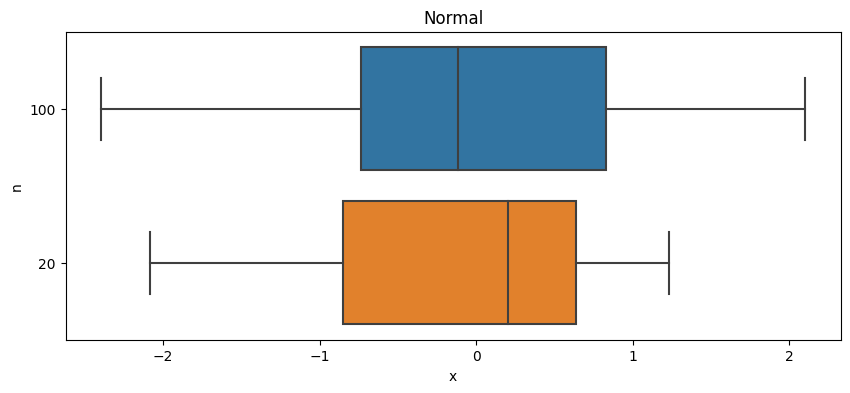
\includegraphics[width=\textwidth]{tasks/3/res/1.png}
		\caption{Нормальное распределение}
	\end{center}
\end{figure}

\begin{figure}[H]
	\begin{center}
		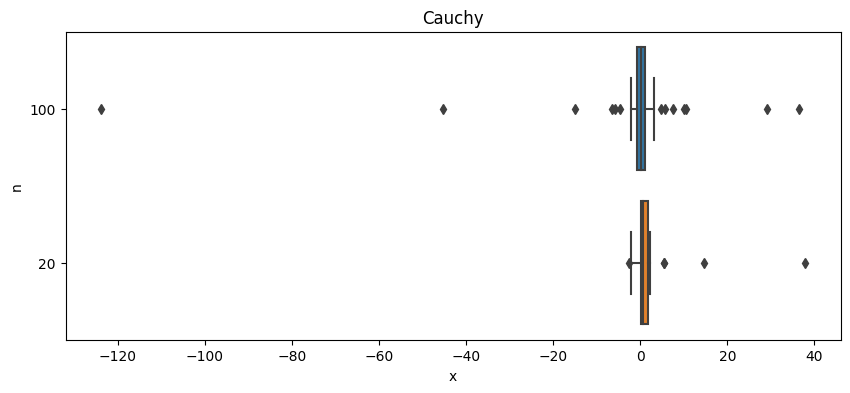
\includegraphics[width=\textwidth]{tasks/3/res/2.png}
		\caption{Распределение Коши}
	\end{center}
\end{figure}

\begin{figure}[H]
	\begin{center}
		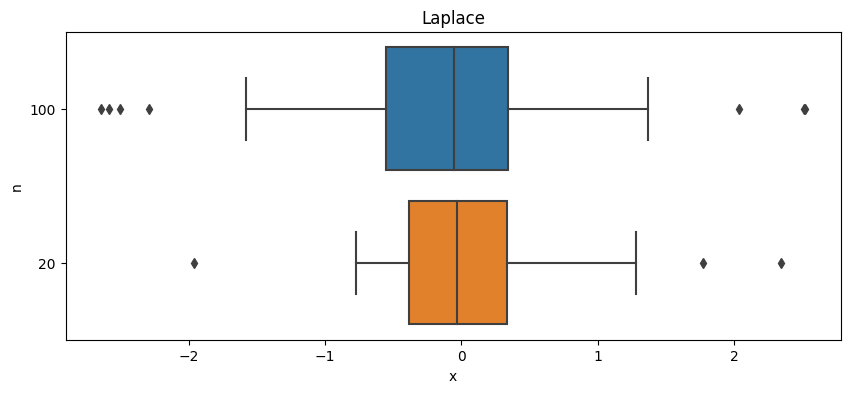
\includegraphics[width=\textwidth]{tasks/3/res/3.png}
		\caption{Распределение Лапласа}
	\end{center}
\end{figure}

\begin{figure}[H]
	\begin{center}
		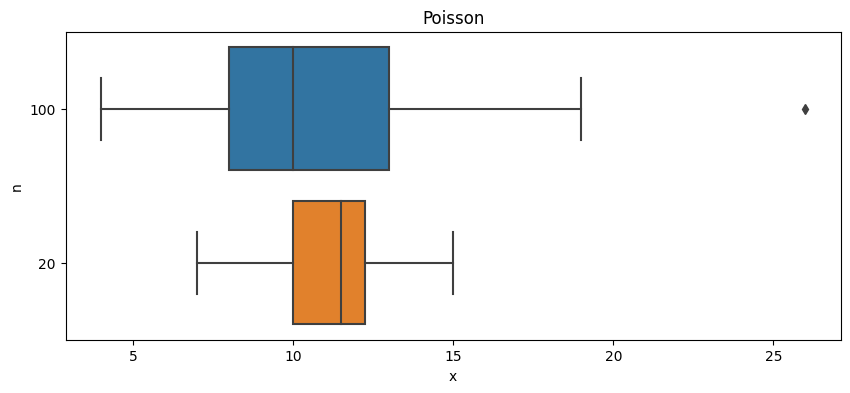
\includegraphics[width=\textwidth]{tasks/3/res/4.png}
		\caption{Распределение Пуассона}
	\end{center}
\end{figure}

\begin{figure}[H]
	\begin{center}
		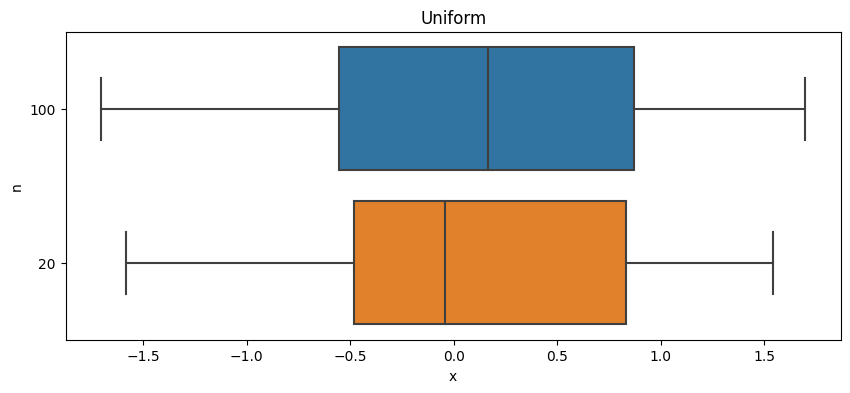
\includegraphics[width=\textwidth]{tasks/3/res/5.png}
		\caption{Равномерное распределениеы}
	\end{center}
\end{figure}


\subsection{Доля выбросов}
Выборка случайна, поэтому в качестве оценки рассеяния можно взять дисперсию пуассоновского потока: $D_n \approx \sqrt{n}$ \newline
Доля $p_n = D_n / n = 1 / \sqrt{n}$ \newline
Доля $n = 20$: $p_n = 1 / \sqrt{20}$ - примерно 0.2 или 20\% \newline
Доля $n = 100$: $p_n = 1 / 10$ - 0.1 или 10\% \newline
Из этого можно решить, сколько знаков оставлять в доле выбросов. \newline

\begin{table}[H]
	\centering
	\begin{tabular}[t]{|c|c|}
		\hline
		Выборка         & Доля выбросов \\
		\hline
		Normal n = 20   & 0.02          \\
		\hline
		Normal n = 100  & 0.01          \\
		\hline
		Cauchy n = 20   & 0.15          \\
		\hline
		Cauchy n = 100  & 0.16          \\
		\hline
		Laplace n = 20  & 0.08          \\
		\hline
		Laplace n = 100 & 0.07          \\
		\hline
		Poisson n = 20  & 0.02          \\
		\hline
		Poisson n = 100 & 0.01          \\
		\hline
		Uniform n = 20  & 0.0           \\
		\hline
		Uniform n = 100 & 0.0           \\
		\hline
	\end{tabular}
	\caption{Доля выбросов}
\end{table}

\subsection{Теоретическая вероятность выбросов}
\begin{table}[H]
	\centering
	\begin{tabular}[t]{|c|c|c|c|c|c|}
		\hline
		Распределение             & $Q_1^T$ & $Q_3^T$ & $X_1^T$~\eqref{eq:BoxBorders} & $X_2^T$~\eqref{eq:BoxBorders} & $P_B^T$~\eqref{eq:ProbabilityOutliersContinuousDistributions}~\eqref{eq:ProbabilityOutliersDiscreteDistributions} \\
		\hline
		Нормальное распределение  & -0.674  & 0.674   & -2.698  & 2.698   & 0.007   \\
		\hline
		Распределение Коши        & -1      & 1       & -4      & 4       & 0.156   \\
		\hline
		Распределение Лапласа     & -0.490  & 0.490   & -1.961  & 1.961   & 0.063   \\
		\hline
		Распределение Пуассона    & 8       & 12      & 2       & 18      & 0.008   \\
		\hline
		Равномерное распределение & -0.866  & 0.866   & -3.464  & 3.464   & 0       \\
		\hline
	\end{tabular}
	\caption{Теоретическая вероятность выбросов}
\end{table}